\section{Introduction}
\label{sec:intro}
Digital twin (DT) models provide synchronized virtual representations for monitoring, prediction, and control in industrial, wireless, and networked computing systems \cite{tao2019dt,khan2022wirelessdt,mihai2022dtsurvey,xu2023dtiot,wu2021dtnetwork}. After deployment, these models must remain aligned with operating conditions that evolve over time. Newly accumulated monitoring data enable maintenance, but they may reflect legitimate workload and resource changes or unreliable observations caused by measurement noise, stale data, communication faults, or manipulation. Directly updating the deployed model can therefore improve adaptation while also replacing a stable state with a degraded one. Figure~\ref{fig:problem-setting} illustrates this maintenance setting.

\begin{figure}[t]
\centering
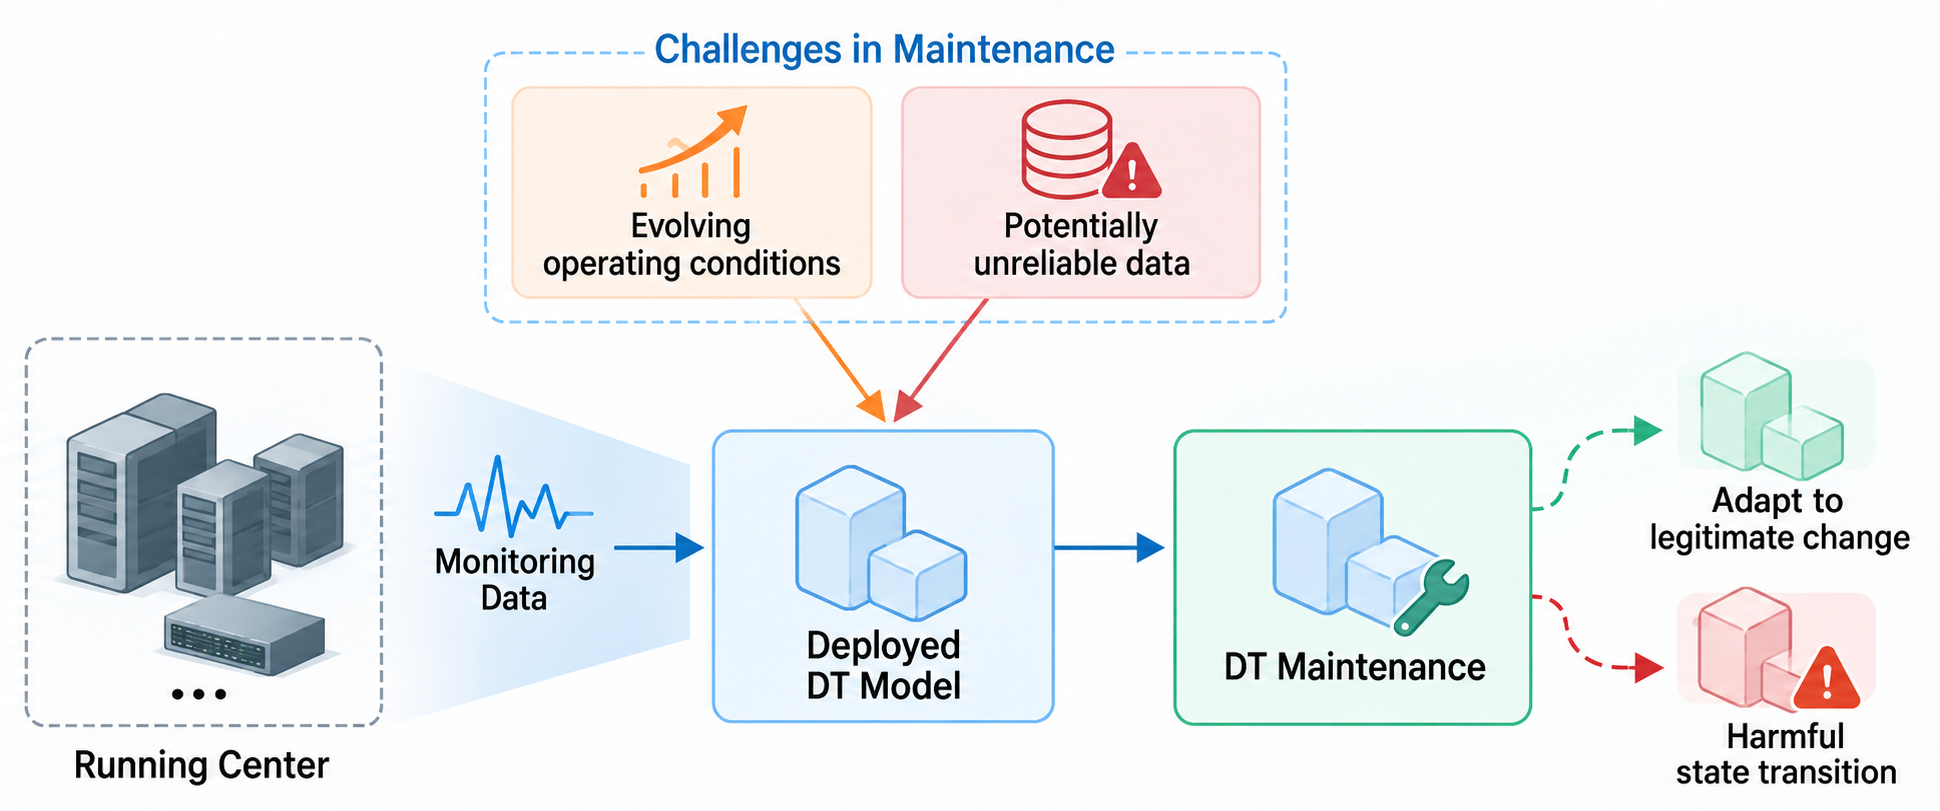
\includegraphics[width=0.88\textwidth]{fig1_problem_setting.pdf}
\caption{Problem setting for continual DT maintenance under evolving operating conditions and potentially unreliable monitoring data.}
\label{fig:problem-setting}
\end{figure}

Existing DT updating and synchronization methods maintain physical--virtual consistency as system conditions change \cite{li2024dtcl,rodriguez2023updating,amad2025calmdt}, while broader network-DT studies emphasize adaptive modeling and lifecycle synchronization \cite{qin2024dtnn,hakiri2024dtsurvey}. Continual-learning methods address sequential adaptation and knowledge retention, and reliability-oriented methods detect or mitigate unreliable observations before model modification. However, these lines of work do not explicitly treat post-adaptation state replacement as a separate deployment decision. When benign operating changes and unreliable observations coexist, successful adaptation on available maintenance data does not guarantee a beneficial deployed-state transition. The remaining challenge is therefore to make candidate-to-deployed state transitions reliable while retaining useful adaptation.

To address this challenge, we propose RAVM-DT, a verification-guided continual maintenance algorithm for deployed DT models. At each maintenance stage, RAVM-DT adapts the current model using update data to form a candidate, compares that candidate with the deployed state using paired recent and bounded historical verification evidence, and commits it only when both evidence criteria support replacement. Bounding the historical evidence horizon limits the influence of obsolete operating regimes while preserving temporally distinct evidence against harmful replacement.

The main contributions are as follows.
\begin{itemize}
    \item \textbf{State-transition formulation for continual DT maintenance.} We formulate maintenance under evolving and potentially unreliable monitoring data as repeated candidate-to-deployed state transitions, characterized by lifecycle loss, harmful-transition frequency, and harmful-transition downside.
    \item \textbf{Verification-guided selective state transition.} RAVM-DT separates candidate adaptation from deployment commitment and uses paired recent and bounded historical evidence to decide whether to commit or retain the current state.
    \item \textbf{Evaluation of the safety--utility--plasticity trade-off.} We evaluate the fixed RAVM-DT configuration under benign drift, multiple corruption patterns and severities, mechanism variants, model architectures, prediction horizons, maintenance cost, and an external production workload trace.
\end{itemize}

The remainder of this paper is organized as follows. Section~\ref{sec:related} reviews related work. Section~\ref{sec:problem} defines the problem, Section~\ref{sec:method} presents RAVM-DT, Section~\ref{sec:experiments} reports the evaluation, and Section~\ref{sec:conclusion} concludes the paper.
